% !TEX encoding = UTF-8 Unicode
% -*- coding: UTF-8; -*-
% vim: set fenc=utf-8

% REVIEW: {referencial, embasamento} teórico
\chapter{Referencial Teórico}%
\label{chap:referencial-teorico}

Nesse capítulo serão abordados alguns conceitos e a terminologia que será utilizada ao longo do trabalho. Parte desse conteúdo, que será referenciado por~\cite{silva2015propostadoutorado}, é baseada na proposta de doutorado do \textsf{M. Sc. Vítor Silva Sousa}, um dos orientadores desse trabalho.

\perrotta{check bibliography: dataflow technical report (key is silvatechnicalreport)}

\section{Simulação Computacional}

Uma \textbf{simulação computacional}, também chamada de \textbf{simulação científica}, é um ``método de abstração e sistematização do processo experimental ou parte dele''~\cite{silva2015propostadoutorado,dias2015data}. Ela emergiu como um meio de executar experimentos científicos em ambientes computacionais~\cite{ogasawara2011algebraic}, e consiste de um ou vários programas \textit{ad-hoc} de simulação específicos, sendo representados como \textit{atividades} em um \textit{workflow}; tais atividades, em particular, são encadeadas para formar uma dependência de dados entre as mesmas, isto é, de forma que os dados produzidos por uma delas sejam consumidos pela outra.

Uma simulação computacional pode ser representada através de um fluxo de dados (elucidado na~\autoref{sec:dataflow}), no qual ``as atividades correspondem às transformações de dados e as dependências de dados correspondem ao fluxo de dados entre duas transformações de dados''~\cite{silva2015propostadoutorado,ogasawara2011algebraic}. Uma \textbf{atividade} é definida como um componente do \textit{workflow} que é capaz de executar programas, com parâmetros de entrada e de saída, os quais são utilizados para representar dependências entre cada uma das atividades.

% REVIEW: map, reduce, etc @ http://vldb.org/pvldb/vol4/p1328-ogasawara.pdf ??

\perrotta{Expandir SGWfC}.

\subsection{SGWfC}

Devido à complexidade das simulações computacionais, um SGWfC --- Sistema de Gerência de \textit{Workflows} Científicos ---, costuma ser empregado para gerenciá-las; em particular, aspectos tais como a composição (\textit{i.e.}, definição da estrutura do fluxo de dados), a execução e a análise (\textit{i.e.}, mecanismo para processamento de consultas e~/~ou ferramentas de visualização) de simulações são administrados pelo SGWfC~\cite{silva2015propostadoutorado}. Eles também proveem abstração para o usuário.

Exemplos de SGWfCs incluem o Chiron~\cite{ogasawara2013chiron}, o Kepler~\cite{ludascher2006scientific} e o Pegasus~\cite{deelman2005pegasus}.

% REVIEW: dataflow
\section{Fluxo de dados}%
\label{sec:dataflow}

\subsection{Conceito de fluxo de dados} % REVIEW: escrever apenas 'conceito'?

Um \textbf{fluxo de dados} (do inglês \textit{dataflow}) é modelado como um grafo direcionado acíclico (DAG), no qual os vértices (nós) representam as atividades / transformações de uma simulação computacional, e as arestas representam o fluxo de dados (conjuntos de dados) entre as atividades~\cite{ogasawara2011algebraic}.

Formalmente, uma especificação de fluxo de dados \( D_F \) é definida como \[ D_F = (T, S, \Phi) \] onde:
\begin{itemize}
    \item \( T = \{t_1, t_2, \ldots, t_{\alpha}\} \) é um conjunto de transformações
    \item \( S = \{s_1, s_2, \ldots, t_{\beta}\} \) é um conjunto de dados
    \item \( \Phi = \{\phi_1, \phi_2, \ldots, \phi_{\gamma}\} \) é um conjunto de dependência de dados
\end{itemize}

\missingfigure{Exemplo de -> o ->, i.e., transformação com dataset de entrada e de saída}

\perrotta{Acho que falta definir o que é uma transformação.}

\subsection{Dependência de dados}

Uma especificação de dependência de dados \( \phi \) é definida como \[ \phi = (s, t_{\textrm{previous}}, t_{\textrm{next}}) \] onde:
\begin{itemize}
    \item \( s \) é um conjunto de dados
    \item \( t_{\textup{previous}} \) é a transformação que {\bf produz} dados para o conjunto de dados \( s \)
    \item \( t_{\textup{next}} \) é a transformação que {\bf consome} dados do conjunto de dados \( s \)
\end{itemize}

\subsection{Conjunto de dados}

A especificação de um conjunto de dados \( s \) é dada por \[ s = (A, C) \] onde:
\begin{itemize}
    \item \( A = \{a_1, a_2, \ldots, a_{\delta} \} \; \vdots{} \; \{ a_i \mid i \in \{1, 2, \ldots, \delta \} \} \) é atributo
    \item \( C = \{c_1, c_2, \ldots, c_{\zeta} \} \; \vdots{} \; \{ c_i \mid i \in \{1, 2, \ldots, \zeta \} \} \) é coleção de dados
\end{itemize}

\subsection{Atributo}

Um atributo é especificado da seguinte forma: \[ a = (\textrm{nome},\textrm{tipo}) \therefore \textrm{tipo} = \{\textup{inteiro}, \textup{ponto flutuante}, \textup{texto}, \textup{arquivo}\} \]

\subsection{Coleção de dados}

Uma coleção de dados é definida como \[ c = \{ i_1, i_2, \ldots, i_{\eta} \} \; \vdots \; \{ i_j \mid j \in \{ 1, 2, \ldots, \eta \} \} \] é item de dados

\subsection{Item de dados}

A especificação de um item de dados é dada por \[ i = (s, T^{\ast}_{\textrm{previous}}, T^{\ast}_{\textrm{next}}, e) \] onde:

\begin{itemize}
    \item \( s \) é um conjunto de dados
    \item \( T^{\ast}_{\textrm{previous}} \) é o conjunto com todas as instâncias de todas as transformações que são responsáveis por gerar \( i \)
    \item \( T^{\ast}_{\textrm{next}} \) é o conjunto com todas as instâncias de todas as transformações que consomem \( i \)
    \item \( e \) é um elemento de dados
\end{itemize}

\subsection{Elemento de dados}

Um elemento de dados é definido como

\[ e = \{ v_1, v_2, \ldots, v_{\theta} \} \therefore \#(s.A) = \#(e) \]
\[ v_{\theta} \; \textrm{é o valor do atributo} \; a_{\theta} \; \textrm{de um item de dados do conjunto de dados} \; s \]

onde \( \#(S) \) representa a cardinalidade do conjunto \( S \), i.e.\ a quantidade de elementos presentes no mesmo.

\subsection{Um exemplo}%
\label{sec:um-exemplo-de-dataflow}

Para ilustrar as definições e especificações da \autoref{sec:dataflow}, vamos utilizar uma pequena amostra do conjunto de dados de sedimentação. Na \autoref{fig:example-dataflow-specification} \perrotta{expandir comentário sobre a figura}

\begin{figure}[ht]
    \centering
    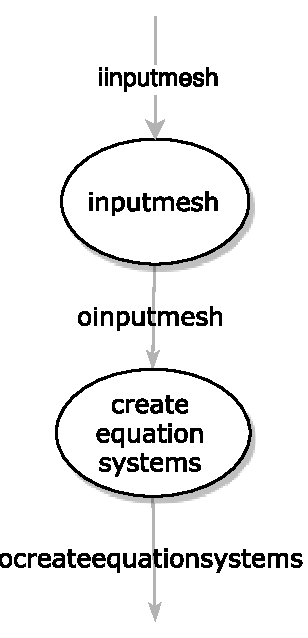
\includegraphics[width=0.35\textwidth]{img/example-dataflow-specification}
    \caption[Exemplo de especificação de fluxo de dados]{Exemplo de especificação de fluxo de dados, com duas transformações e três conjuntos de dados.}%
    \label{fig:example-dataflow-specification}
\end{figure}

\missingfigure{Incluir um exemplo, com figuras, de um pequeno dataflow.}

\[
\begin{aligned}
D_F = && (T, S, \Phi) \\
T = && \{ \textrm{inputmesh} \} \\
S = && \{ \textrm{iinputmesh}, \textrm{oinputmesh} \} \\
\Phi = && \{ (\textrm{nil}, \textrm{iinputmesh}, \textrm{inputmesh}),
(\textrm{inputmesh}, \textrm{oinputmesh}, \textrm{nil})
\} \\
\end{aligned}
\]

\perrotta{Capítulo 02 --- misc}

%%%%%%%%%%%%%%%%%%%%%%
% Simulações computacionais
% (OK) Fluxo de dados = dataflow - definições {d,n}o outro google docs
\section{Proveniência de dados}

% REVIEW: {conceito, definição}
\subsection{Conceito de proveniência}  % REVIEW: escrever apenas 'conceito'?

% upstream: http://www.aulete.com.br/proveni%C3%AAncia
O dicionário Aulete Digital~\cite{auletedigitalonline} define \textbf{proveniência} como
``lugar de onde alguém ou alguma coisa provém; origem; FONTE;''. Em experimentos científicos, a proveniência nos ajuda a interpretar e entender resultados. Através da examinação e da cadeia de passos que criaram um certo resultado, nós podemos verificar que o experimento foi: (i) realizado de acordo com os procedimentos aceitáveis; (ii) inspecionar as suas entradas; e, em alguns casos, (iii) reproduzir os mesmos resultados~\cite{freire2008provenance}.

Questões básicas sobre dados científicos podem ser respondidas através do conhecimento e da introspecção de sua proveniência, tais como

\begin{enumerate}
    \item quem criou o dado, e quando foi essa criação?
    \item quem modificou o dado, e quando essa modificação ocorreu?
    \item que processo criou o dado?
    \item que outros dados foram produzidos a partir dos dados originais?
\end{enumerate}

Um dos componentes mais importantes que podemos obter com proveniência são suas informações sobre \textbf{causalidade}, isto é, a relação de dados de entrada que, associados a um processo, levam a um determinado conjunto de dados de saída~\cite{freire2008provenance}. A causalidade pode ser representada através de \textit{workflows} e de grafos --- onde nós correspondem a processos e arestas correspondem a dados científicos ---, como no exemplo da \autoref{sec:um-exemplo-de-dataflow}.

Um segundo exemplo relevante de componente de proveniência são as informações definidas e providas pelo usuário, as quais não podem ser capturadas automaticamente~\cite{freire2008provenance}. Esse tipo de informação é usualmente provido em níveis de granularidade arbitrários através de anotações e observações do usuário.

\subsection{Categorias de dados de proveniência}

Existem dois tipos de proveniência para \textit{workflows} científicos: \textbf{prospectiva} e \textbf{retrospectiva}~\cite{murta2014noworkflow,freire2008provenance}:

\begin{itemize}
% murta2014noworkflow ++ freire2008provenance
    \item A \textbf{proveniência prospectiva} captura a especificação e a estrutura de uma tarefa computacional --- por exemplo, um \textit{script}, ou um \textit{workflow} --- e associa a ela os passos que precisam ser seguidos para gerar um conjunto de dados. Ela corresponde à definição de um \textit{workflow} e ao seu grafo de atividades, processos e de dados científicos relacionados.
% murta2014noworkflow ++ freire2008provenance
    \item Por outro lado, a \textbf{proveniência retrospectiva} captura não apenas os passos executados de uma tarefa computacional, mas também informações relacionadas ao ambiente e tempo de execução da mesma - por exemplo, quais parâmetros foram passados aos programas, qual \abbrev{PID}{Process ID} processo (PID) do sistema operacional foi executado, por quem o PID foi executado, qual foi a duração total (incluindo seu instante de início e de fim) do mesmo, ou quais variáveis de ambiente do sistema operacional estavam definidas. Sua estrutura do grafos é similar à da proveniência prospectiva.
\end{itemize}

Através dos dois tipos citados de proveniência, um SGWfC é capaz de orquestrar e prover diferentes níveis de abstração para a execução de uma simulação científica~\cite{murta2014noworkflow}, os quais são inexistentes em programas \textit{ad-hoc} tais como \textit{scripts}. Além disso, mecanismos básicos de captura de proveniência podem ser classificados em três classes, de acordo com o tipo de captura em que são baseados~\cite{freire2008provenance}:

\begin{itemize}
    \item \textit{workflows}: SGWfCs, por exemplo, sistemas tais como Kepler~\cite{ludascher2006scientific} e Taverna~\cite{hull2006taverna};
    \item processos: PID, comunicação entre processos (IPC);
    \item sistema operacional: por exemplo, através de chamadas de sistema.
\end{itemize}

Ademais, a captura de proveniência de dados pode ser realizada de duas formas distintas, \textit{offline} e \textit{online}~\cite{silva2015propostadoutorado}. A captura \textit{offline} consiste em armazenar os dados de uma simulação científica em um determinado repositório logo \textbf{após} a execução da mesma --- por exemplo, como realizado pelo Kepler~\cite{ludascher2006scientific}. Em contrapartida, a captura \textit{online} consiste na obtenção e no armazenamento de dados \textbf{em tempo de execução}, como realizado no Pegasus~\cite{deelman2005pegasus} e no Swift/T~\cite{zhao2007swift}.
% /\ REVIEW: Swift ou Swift/T? Citação está correta?

Uma simples observação é que o desempenho da captura de proveniência \textit{online} tende a ser ligeiramente pior do que a \textit{offline}, devido à possível sobrecarga do armazenamento de dados de proveniência concorrentemente ao processamento dos programas de simulação. Em outra perspectiva, vale enfatizar que a captura \textit{online} é mais flexível e tem um potencial analítico maior, pois permite que os usuários realizem consultas mesmo antes do término da simulação, o que possui um valor inestimável, uma vez que simulações computacionais são comumente realizadas em larga escala sendo, portanto, custosas e demoradas.

\subsubsection{Um exemplo}

Para ilustrar a diferença entre os dois tipos de proveniência apresentados, considere o clássico exemplo de contagem de palavras (\textit{word counting}), no qual o conjunto de dados inicial é um arquivo de texto em \abbrev{ASCII}{American Standard Code for Information Interchange} ASCII\footnote{Cujo objetivo é obter a ordem decrescente de frequência das palavras que aparecem no texto}. A primeira tarefa de processamento é a leitura e subsequente análise do arquivo de texto a fim de extrair palavras do mesmo. A segunda etapa é realizar a contagem das palavras a partir da lista de palavras obtida no passo anterior. Finalmente, o último passo de processamento é ordenar em ordem descrescente a frequência de palavras obtida no passo anterior.

A proveniência prospectiva desse experimento poderia ser representada através do grafo da \autoref{fig:word-count-prospective}. Por outro lado, a proveniência retrospectiva do último passo (ordenação) poderia ter capturado em tempo de execução algumas das informações presentes na \autoref{tab:word-count-retrospective}.

\begin{figure}[ht]
    \centering
    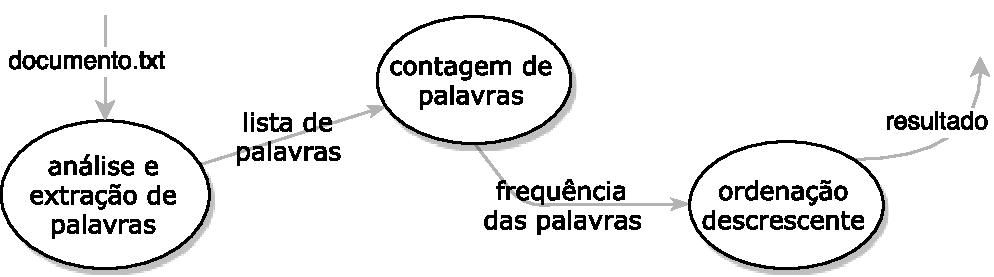
\includegraphics[width=\textwidth]{img/word-count-prospective}
    \caption[Proveniência prospectiva do exemplo de contagem de palavras]{Proveniência prospectiva do exemplo de contagem de palavras.}%
    \label{fig:word-count-prospective}
\end{figure}

\begin{table}[ht]
    \centering
    \begin{tabular}{r|l}
        \hline
        \textit{Timestamp} de início & 2017-06-25 03:11:05.231                         \\
        \textit{Timestamp} de fim    & 2017-06-25 03:11:09.586                         \\
        PID                          & 4671                                            \\
        Linha de comando             & \texttt{./sort --order=desc --in=freq-list.csv} \\
        Variáveis de ambiente        & \texttt{PWD=/home/tperrotta;PATH=/usr/bin:/bin} \\
        Usuário                      & tperrotta                                       \\
        \hline
    \end{tabular}
    \caption[Proveniência retrospectiva do exemplo de contagem de palavras]{Proveniência retrospectiva do exemplo de contagem de palavras da etapa de ordenação decrescente.}%
    \label{tab:word-count-retrospective}
\end{table}

% REVIEW: \section{Gerência do fluxo de dados}
\section{Rastreamento de dados de proveniência}

\subsection{Físico}

O \textbf{rastreamento físico} de dados de proveniência gerencia a proveniência de \emph{elementos de dados} individuais, isto é, num nível de granularidade fino. Nessa abordagem é necessário etiquetar cada elemento de dado com identificadores, de forma a habilitar o gerenciamento do fluxo de dados. Esse tipo de proveniência captura muitos detalhes, os quais podem ser úteis na depuração de simulações devido ao seu gerenciamento fino de \perrotta[elementos de dados.]{citation needed: dataflow technical report from Victor et al}

\subsection{Lógico}

O \textbf{rastreamento lógico} de dados de proveniência, de forma análoga ao rastreamento físico, também rastreia o fluxo de elementos de dados, só que a captura é realizada através de \emph{transformações}, em vez de elementos de dados. Dessa maneira, menos dados de proveniência precisam ser armazenados, já que um fluxo de dados costuma ter bem menos transformações do que elementos de dados. Além disso, o rastreamento lógico pode ser \emph{automaticamente} derivado das especificações das transformações de dados, uma vez que elas já apresentam propriedades sobre conjuntos de dados consumidos e produzidos~\cite{ikeda2013logical}.

\perrotta{citation needed: dataflow technical report from Victor et al}

\subsubsection{Exemplo}

\perrotta{Exemplo para ilustrar: diferença entre físico e lógico}
\missingfigure{Exemplo para ilustrar: diferença entre físico e lógico}

% Mecanismos para processamento de consultas